% Capítulo: Background
% Codificación: UTF-8

\chapter{Background}
\label{chap:background}

This chapter provides the background for the thesis in four parts.
Section~\ref{sec:isa-specs} introduces instruction set architectures, the
documents that specify them, and the formal, executable specifications that
have been developed to complement those documents. Section~\ref{sec:pisa} introduces
PISA, Intel's new virtual ISA for its GPUs, and gives an overview of the
execution and memory models it defines. Section~\ref{sec:gpu-isa-state} presents the work done on GPU ISAs
and how they are specified today. Section~\ref{sec:asl}
introduces ASL, the language in which ARM writes its executable specifications.

\section{ISA Specifications}
\label{sec:isa-specs}

An instruction set architecture (ISA) is the interface between a
processor and the software that runs on it. It specifies what the
processor can do: which instructions it executes and how they are
encoded, which registers it has, how memory is addressed, and how it
communicates with devices. ISA specifications have traditionally been
written as documents. As processors have grown more complex, so have
these documents, and keeping them correct has become a troublesome task. For example, the instruction set reference for Intel's 64 and IA-32
architectures runs to more than 2500 pages~\cite{intel-isa}. The traditional role of the 
specification is to serve as reference documentation. 
Good ISA documentation is essential during the processor's design and
for the development of software tools related to the ISA, such as compilers and simulators. The ISA specification is the single source of truth about the processor's
architecture, and it is read by users from many backgrounds: the architects
who write and maintain it, compiler engineers looking for optimization
opportunities, and external researchers making correctness claims about the
processor's behavior and guarantees. The specification must be accessible to
all of them.

These consumers, however, do not only read the specification: they also
build software that must agree with it. Compiler engineers consult the
specification for each instruction's encoding and implement it in the
compiler backend. Before a processor is manufactured, engineers rely on
simulators to verify the correctness of the generated code, and they build
those simulators from the specification's description of each instruction's
semantics and its effect on the overall architecture. 
Each of these consumers must translate the original specification into their own
tools, by hand, and keep it up to date against the latest changes. Each of these
translations is an opportunity
for the interpretations to disagree with each other and with the document
itself. This has been the motivation for some processor developers to adopt
\emph{machine-readable, mechanized, executable} ISA specifications.

\subsection{Formal and Executable Specifications}
\label{sec:formal-isa}

ARM, besides the usual written document, provides a machine-readable and
executable specification for its A-profile architecture~\cite{arm-spec}. The
machine-readable specification contains the instruction and system register
encodings, written in XML, and the executable specification describes the
instruction semantics. Reid~\cite{reid-trustworthy-specs} describes a five-year project to
transition ARM's v8-A and v8-M specifications from written documents
into trustworthy machine-readable specifications.
Instruction semantics, previously written in an informal C-like pseudocode,
were rewritten in a strongly typed, executable language, the Architecture
Specification Language (ASL). This allowed ARM to fill gaps in the
specification that had been described only in English. For example, the
top-level step of fetching, decoding, and executing an instruction was
written in ASL. Most importantly, the ASL specification could run ARM's test
suites, and doing so found bugs in the reference simulators that followed
the original specification.

ASL has served as the baseline for verification work on the ARM
architecture. Reid et al.\ translated ASL to Verilog to build ISA-Formal, an
end-to-end verification framework that detects bugs in the datapath,
pipeline control, and forwarding and stall logic of processors. Because the
framework works from the translated specification, it scaled to the full
instruction set~\cite{reid-isa-formal}. In later work, Reid simplified ASL
and converted it into verification conditions, expressed as SMT formulas
that the Z3 solver can check. With them he found multiple bugs in both the
natural-language and the machine-readable
specification~\cite{reid-who-guards}.

ASL is not the only specification language in use. Sail, developed by
Armstrong et al.~\cite{isa-semantics}, is a specification language with
characteristics similar to those of ASL. Specifications for RISC-V, MIPS,
CHERI-MIPS, and ARM have been written in Sail. Sail specifications can be
translated for the theorem provers Isabelle/HOL, HOL4, and Coq, and they can
also generate emulators, since Sail maps directly to OCaml and compiles to
C. The ARM ASL specification was translated into Sail and then into Lem, and
with Isabelle/HOL4 the authors found bugs in its translation of virtual to
physical memory addresses. ASL has also begun a second life outside ARM. Intel Labs maintains ASLi, the
ASL interpreter and C backend, and has since developed from it the Intel ISA
Specification Language, an ASL-derived language whose development is led by ASL's
original designer~\cite{intel-isa-tools}.

\subsection{Virtual Instruction Sets}
\label{sec:virtual-isa}

Manufacturers may choose to add a layer of abstraction over their processors
by defining a \emph{virtual} ISA. A virtual instruction set is defined independently of
any particular hardware, and it serves as a stable compilation target that a
virtual machine or just-in-time compiler translates into native code at or
before execution~\cite{adve-llva}.

Decoupling the instruction set from the hardware brings portability, since
software runs across hardware platforms without modification, and forward
compatibility, since software written for one generation continues to run on
the next. Virtual ISAs also serve as an intermediate representation that
carries program information the translator can exploit for optimization on
the target hardware, and they let processor designers adopt new architectural
features without disrupting the existing software
ecosystem~\cite{adve-llva}.

A popular virtual ISA for GPUs is NVIDIA's Parallel Thread Execution
(PTX) ISA~\cite{ptx-isa}, the compilation target of the CUDA platform. PTX is a
published, versioned contract: compilers produce it, shipped binaries embed
it, and drivers translate it across hardware generations, so that programs
compiled to PTX a decade ago still run on current GPUs. It is the interface
NVIDIA exposes to compiler and tool builders rather than the hardware
instruction set beneath it. Intel has recently
published its own virtual ISA for its GPUs, PISA.

\section{Portable ISA Specification}
\label{sec:pisa}
The portable ISA (PISA) specification is a virtual instruction set for Intel's
GPUs. PISA gives compilers a stable target that sits between high-level languages
such as SYCL and C++ and Intel GPUs. It aims to provide ``close to the
metal'' performance comparable to native machine code, and supports advanced
programming through hand-written libraries and inline
assembly~\cite{pisa-spec}.
Intel is also upstreaming an LLVM backend for PISA to the LLVM
project~\cite{pisa-llvm-rfc}, so that programs in OpenCL C and C++
compile to it through Clang. At the time of writing, the backend is
under review as an experimental target~\cite{pisa-llvm-rfc,pisa-llvm-pr}.

\subsection{Execution Model}

The PISA virtual machine defines how kernels are structured, launched and run,
largely following the OpenCL execution model~\cite{pisa-spec,opencl}. 
A kernel is a sequence of PISA instructions executed on the virtual machine.
The host code runs on the CPU and manages which kernels are executed and how
they are organized. When the host code dispatches a kernel for execution,
the virtual machine creates an N-dimensional range (NDRange) of
\emph{work-items} and runs an instance of the kernel for each element of the
range. The host code specifies the total number of work-items to dispatch,
the \emph{global size}. In the NDRange, work-items are grouped into
\emph{work-groups}, whose size, the \emph{local size}, is also specified by
the host code. Each work-group is identified by a unique \emph{group ID},
and within a work-group each work-item is identified by a \emph{local ID}.
Figure~\ref{fig:ndrange} shows this organization. During execution, the
virtual machine further divides each work-group into one or more
\emph{sub-groups}, of a fixed size of 32.

\begin{figure}[htbp]
    \centering
    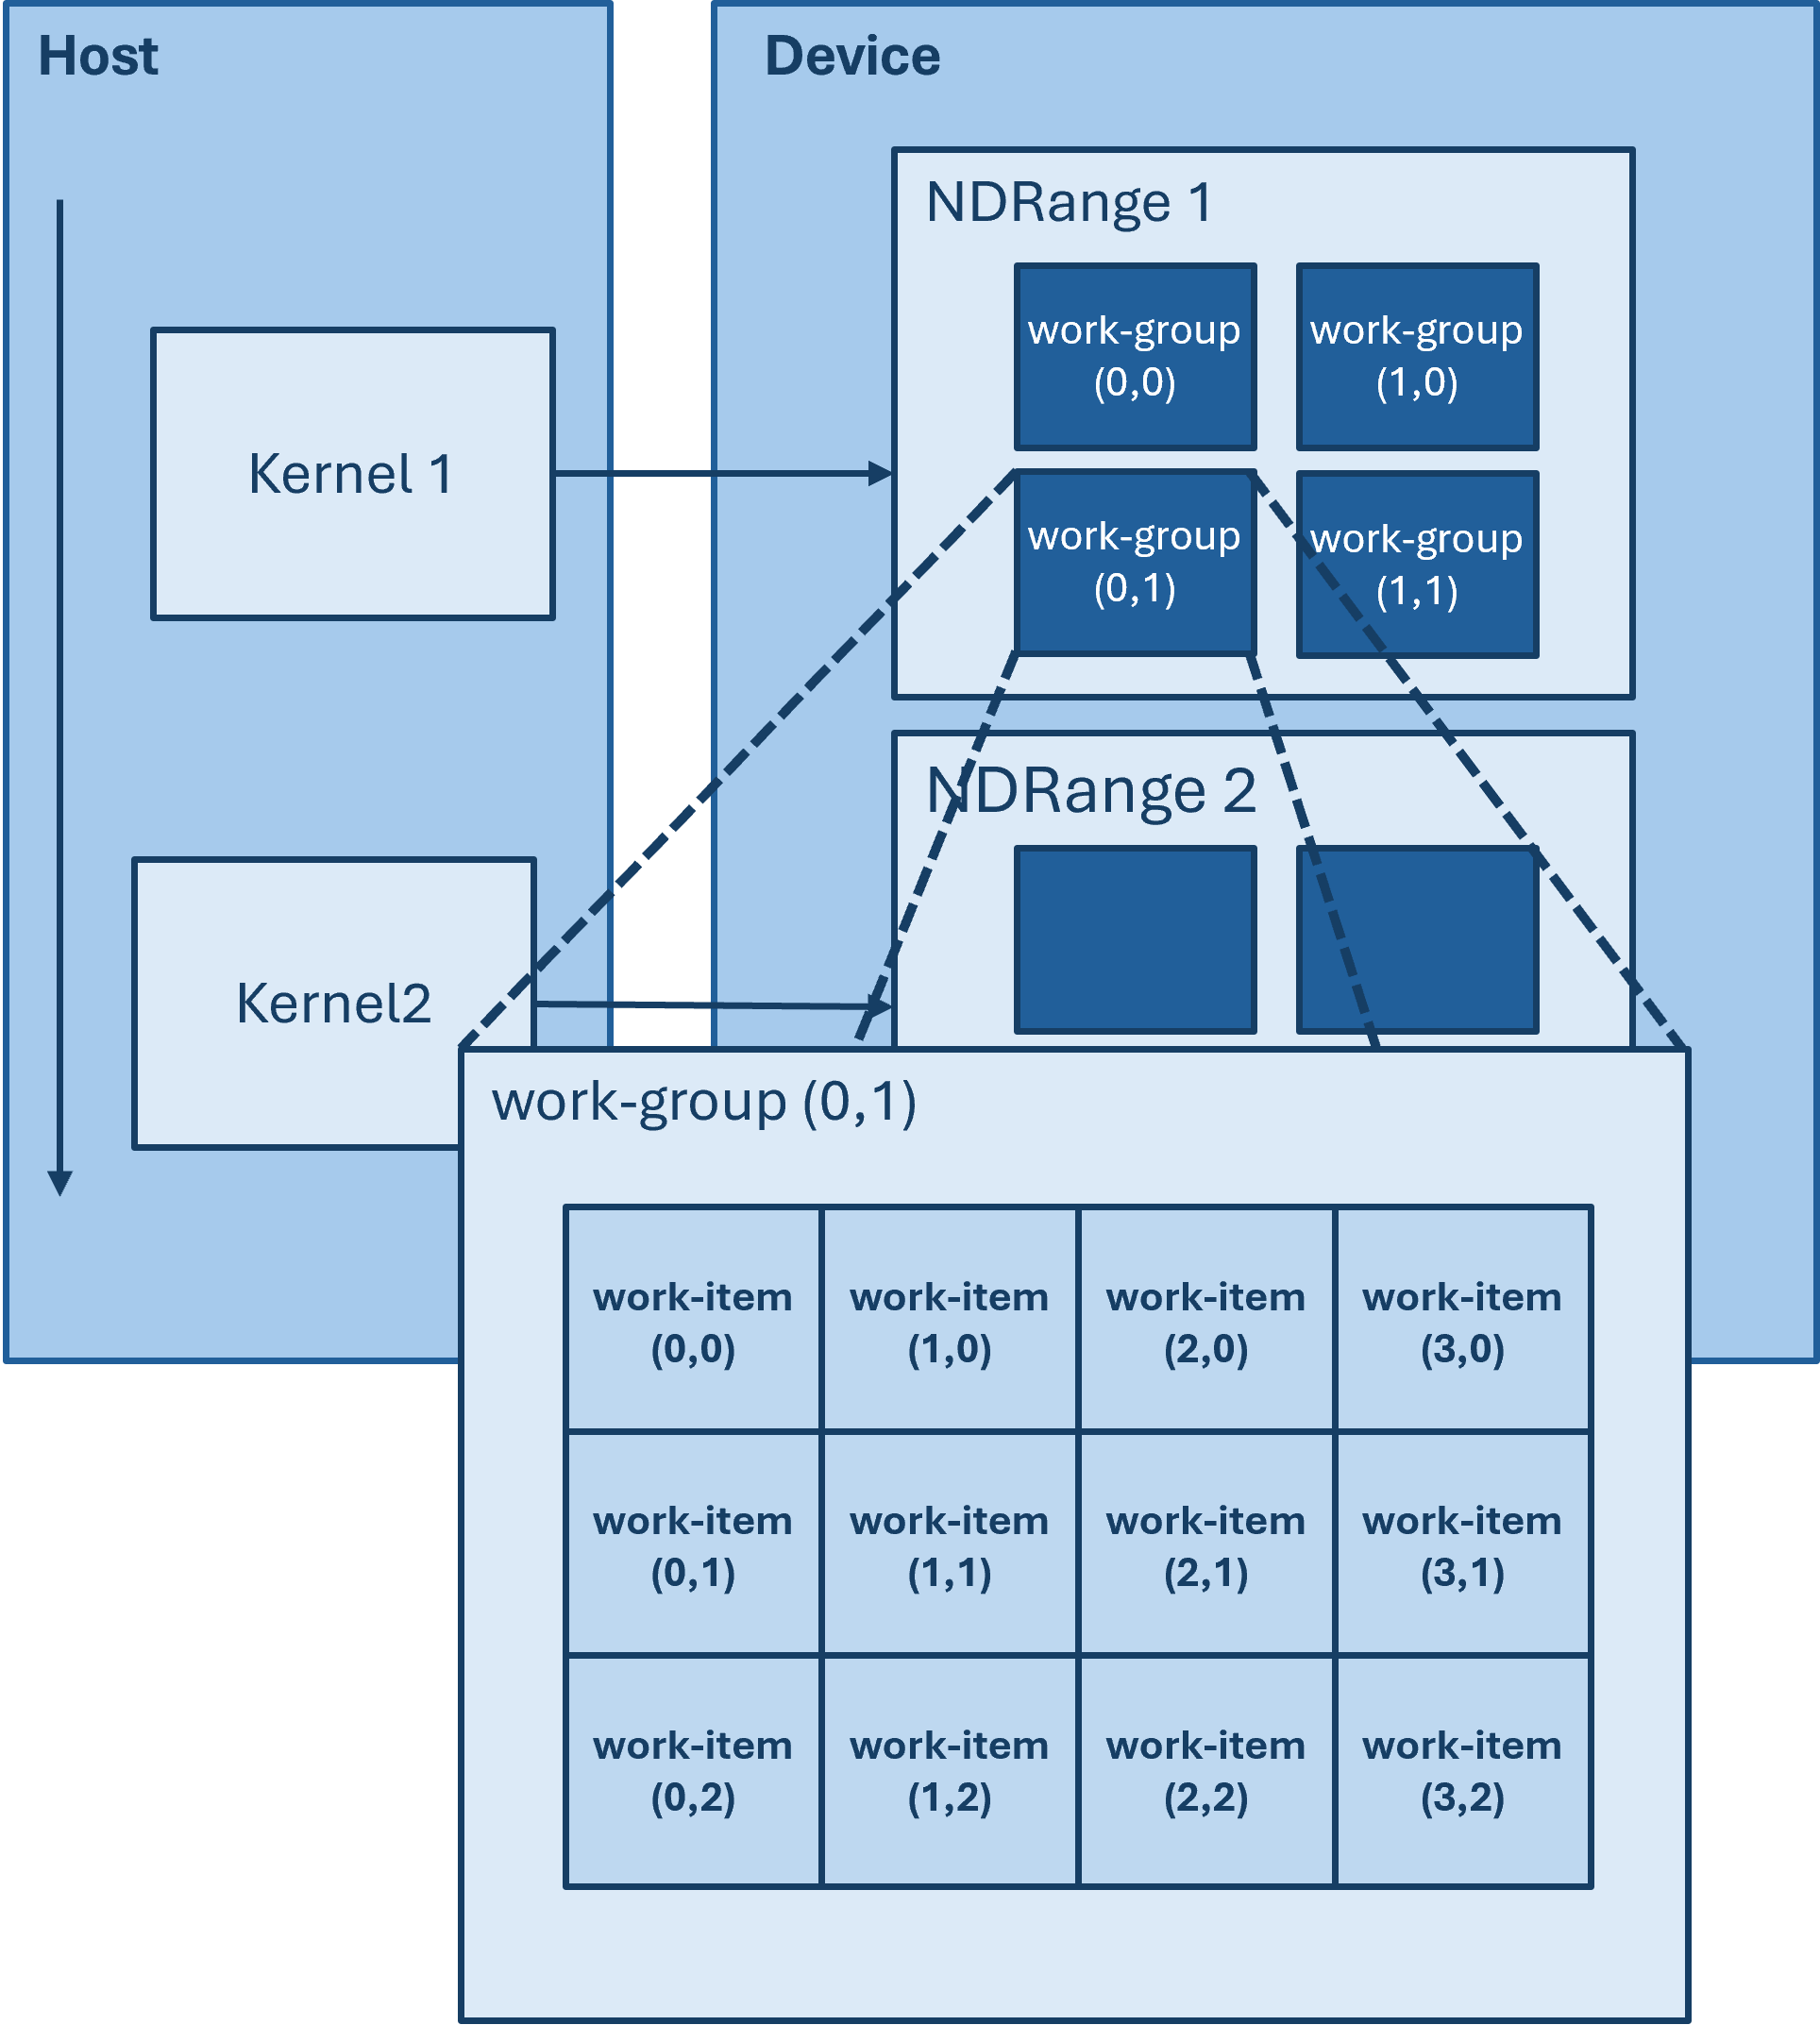
\includegraphics[width=0.6\textwidth]{img/ndrange.png}
    \caption{PISA 2-dimensional NDRange}
    \label{fig:ndrange}
\end{figure}

The virtual machine executes work-groups concurrently, but not necessarily in parallel, and the execution order 
is unspecified. Work-items of the same work-group can synchronize and communicate with each
other. Sub-groups within a work-group make independent forward progress:
unless a sub-group is waiting for another, for example at a work-group
barrier, its execution is not blocked by the other sub-groups. At the sub-group level, work-items can cooperate directly: shuffle
instructions exchange values between lanes, and reduction instructions combine
a value from every work-item into a single result~\cite{pisa-spec}.

PISA does not prescribe how the work-items of a sub-group are executed
together. Like OpenCL, its execution model is compatible with Single
Instruction, Multiple Thread (SIMT) execution, the style in which GPUs
characteristically execute work-items~\cite{lindholm-tesla}. Under SIMT,
the work-items of a sub-group execute the same instruction in lockstep, each
on its own data and registers. Lockstep execution holds only while 
every work-item in the sub-group executes the same instruction. A conditional branch can break 
that condition. If the branch predicate differs across the work-items, some take the branch and
others do not, and the sub-group \emph{diverges}. The machine cannot execute both 
paths at once, so it executes them one after another, each time executing only the 
\emph{active} work-items that belong to the path.  Work-items that do not belong to it are
\emph{inactive}: they do not participate in execution and write no results.
Divergence is confined to the sub-group, since different sub-groups execute
independently regardless of their control flow. Eventually, control flow
reaches a path common to the diverged work-items, where the inactive ones are
reactivated and rejoin execution. This is called \emph{reconvergence}. PISA does not
define a reconvergence mechanism for its virtual machine.

\subsection{Memory Model}

PISA memory is organized hierarchically into address spaces. Each work-item
has its own private memory, visible only to it, which comprises the register
and private spaces: the register space provides fast private storage, and
the private space holds memory objects private to each work-item. Each
work-group has its own shared space, in which the work-items of the
work-group may read and write any variable, synchronizing their accesses
through synchronization instructions. All work-items of an NDRange can
access the global space, which is used to exchange data with the host. A
constant space is also available as a read-only location. The parameter
space holds the kernel arguments passed from the host. It is read-only to the kernel and is written by the runtime 
before the launch. Figure~\ref{fig:memory-hierarchy} shows the spaces and the level of the work-item hierarchy
at which each becomes visible.

\begin{figure}[htbp]
    \centering
    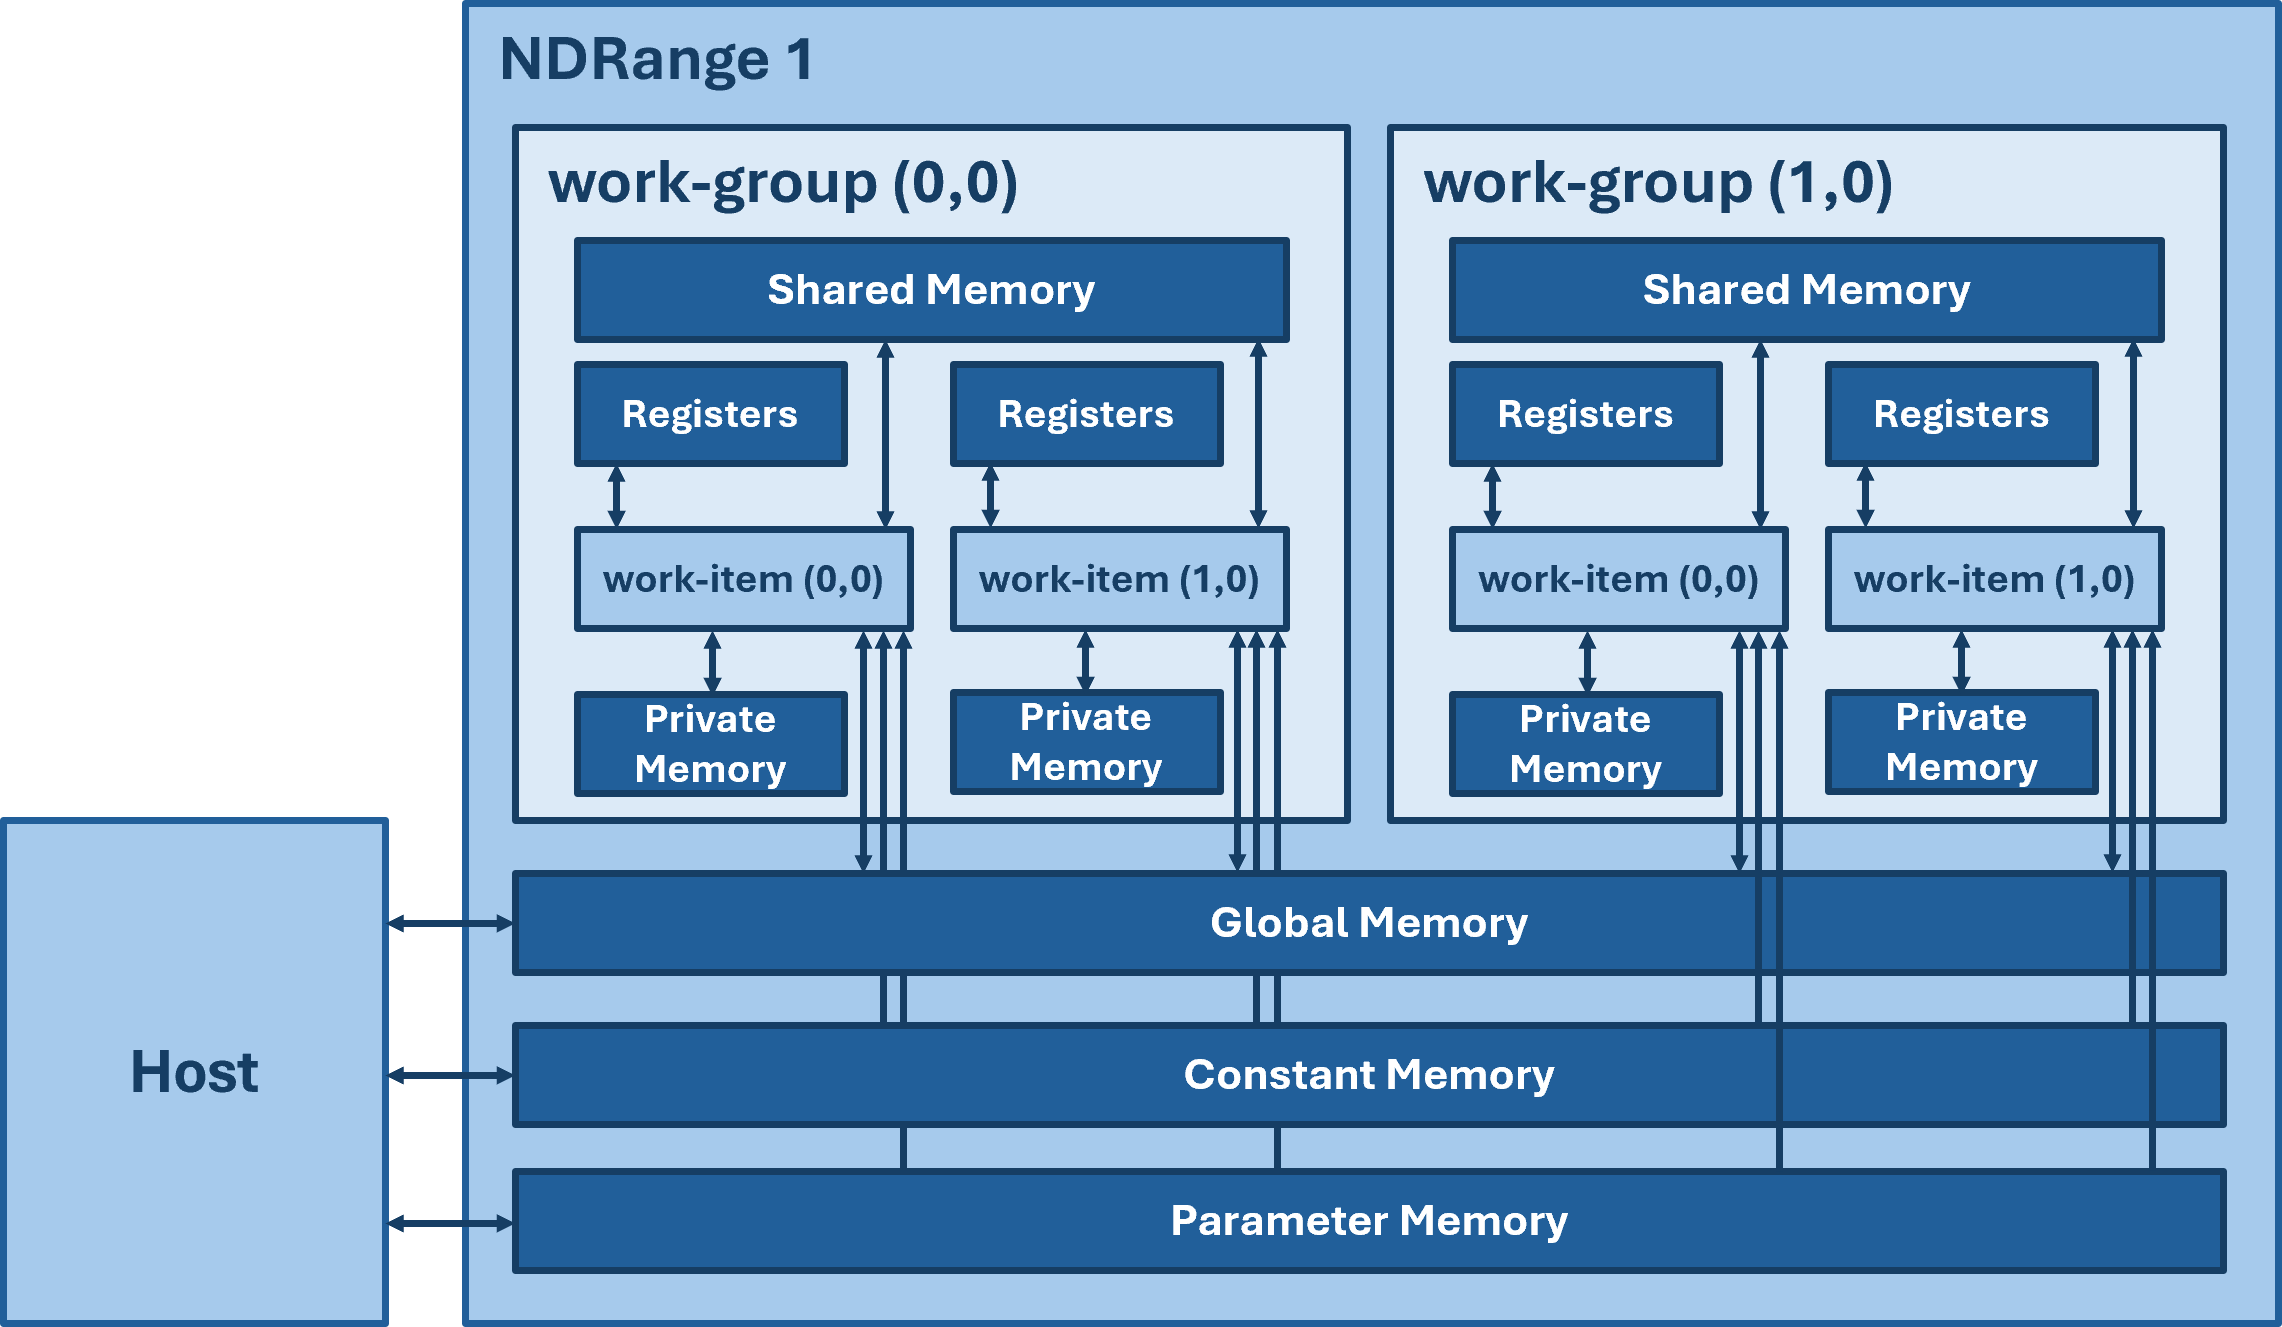
\includegraphics[width=0.6\textwidth]{img/mempisa.png}
    \caption{PISA Memory Hierarchy}
    \label{fig:memory-hierarchy}
\end{figure}

\section{The State of GPU ISA Specifications}
\label{sec:gpu-isa-state}

The GPU virtual ISAs we have presented are specified in prose. Both PTX and
PISA are documented through a natural-language reference
manual~\cite{ptx-isa, pisa-spec}. Both documents are extensive and
carefully written, but carry the risks of a prose specification, and for PTX
these risks have been measured. Lustig et al.\ constructed a formal memory
consistency model for PTX from its documentation~\cite{lustig-ptx-mcm},
and in doing so exposed ambiguities in the published text, together with
cases in which the compiler and the hardware behaved in ways no reasonable
reading of it allowed. Alglave et al.\ approached the same documentation
empirically, testing NVIDIA hardware against the behaviors the CUDA and PTX
manuals describe, and found that the hardware did not comply with its own
published specification~\cite{alglave-gpu-concurrency}. These studies
show that a prose specification can be interpreted in more than one way, and
that the implementation may differ from what has been established in prose.

Parts of GPU execution have been formalized. Habermaier and
Knapp~\cite{habermaier-simt} give a formal semantics of SIMT execution,
with lockstep, divergence, and reconvergence. They prove that a program
executed this way behaves as if its work-items were ordinary threads
interleaved one at a time. Verification tools go one level up and reason
about GPU programs directly. GPUVerify~\cite{gpuverify} takes kernels
written in OpenCL or CUDA and checks them for data races and barrier
divergence. To do so, it defines its own formal model of how a GPU executes
a kernel, encoding the execution model of those programming languages, and
verifies the kernel against it.

There are works on making PTX executable. Performance simulators such as
GPGPU-Sim and its successors~\cite{gpgpu-sim,accel-sim} run PTX
workloads on a model of the GPU microarchitecture to estimate the cost of
architectural decisions. Gutierrez et al.\ measured the cost of this abstraction: because a
virtual ISA hides the hardware by design, simulating at its level
misestimates instruction counts, register contention, and runtime by
wide margins. What a program computes, however, is the same at both
levels. The virtual ISA and the hardware ISA give it the same
semantics, and the results agree~\cite{gutierrez-lost-abstraction}.
Functional emulators work at this level and run PTX for its results alone.
Ocelot~\cite{ocelot} translates PTX for execution on CPUs and other
targets, and Claret Exojo~\cite{claret-ptx-emulation} builds an emulation
library that parses the PTX emitted by the CUDA compiler and emulates the
kernel on the CPU, reproducing the numerical results of the GPU. Both
reproduce the GPU's results from the manual alone.

Each of these lines of work delivers a piece of what a specification would
contain: the ordering of memory operations, the control-flow mechanism, an
execution model to verify programs against, and executable code that
reproduces the hardware's results. Each was built from its authors'
interpretation of the manual, and each is checked against the hardware
rather than the other way around. The same kinds of work exist for ARM,
however, all of them were carried out against one executable
specification, which served as the authority. For PTX, each was carried out
against a separate interpretation of a document. An executable specification
maintained by the ISA's provider would give these works a single reference
to start from.

\section{The Architecture Specification Language}
\label{sec:asl}

The Architecture Specification Language (ASL) is the language in which ARM
writes the pseudocode of its architecture reference manuals. The same source
renders as documentation and runs as a model. ARM publishes a formal
definition of the language, covering its type system and dynamic
semantics~\cite{asl-reference}.

ASL is an imperative language whose types are built around bitvectors of
fixed and parameterized width, alongside unbounded integers, booleans,
enumerations, records, and arrays. Architectural state is declared as
global variables, and instructions are written as functions and procedures
that read and write that state. Listing~\ref{lst:asl-add} shows a
register-to-register addition in this style.

\begin{lstlisting}[language=ASL, caption={An ASL specification of a
register-to-register addition.}, label={lst:asl-add}]
// Architectural state
var R : array[32] of bits(64);

// Instruction semantics
func ADD_reg(d : integer, n : integer, m : integer)
begin
    let operand1 = R[n];
    let operand2 = R[m];
    let result   = operand1 + operand2;
    R[d] = result;
end
\end{lstlisting}

The state is an array of 32 registers of 64 bits, and the instruction is
a procedure over it: two registers are read, added, and the result written to
a third. \lstinline{bits(64)} is a bitvector type, and the type system tracks
widths, so an expression that combines bitvectors of different widths is
rejected rather than silently coerced. A width may also be a parameter of a
function, so that one function describes an instruction for every width it
admits. Memory is provided by the built-in type \lstinline{__RAM(A)}, an
addressable store indexed by addresses of \lstinline{A} bits and read and
written in byte-sized units. A specification declares one such store per
address space it models.

Two implementations execute ASL. ASLRef is the reference implementation of
the language, developed with ARM in the herdtools7 project, whose repository
also holds the sources of the language definition~\cite{aslref}. ASLi, the
ASL interpreter, is Intel Labs' extension of ARM's original open-source
interpreter~\cite{asli}. Beyond interpreting a specification, ASLi compiles
it to C. Its \texttt{asl2c} tool takes a specification together with a
configuration file naming the functions to export, discards everything not
reachable from them, and generates C source and a supporting runtime
library. The exported functions are ordinary C functions, so a program
written in C or C\texttt{++} can initialize the specification's state, run
it, and inspect the result by calling into the generated library. ASLi's
distribution demonstrates this by building a simulator for a small example
architecture from its ASL specification, driven by a hand-written C harness.
The code generator originated in ARM's validation of its specifications,
where interpreting the specification was too slow to run the
architecture's test suites against it~\cite{reid-trustworthy-specs}.